\documentclass[aspectratio=169,11pt]{beamer}
\usepackage[T1]{fontenc}
\usepackage[utf8]{inputenc}
\usepackage[english]{babel}
\usepackage{amsmath,amssymb}
\usepackage{graphicx}
\usepackage{booktabs,tabularx}
\usepackage{xcolor}
\usepackage{tikz}
\usepackage{microtype}

\usetheme{Boadilla}
\usecolortheme{dolphin}
\definecolor{SorbonneNavy}{HTML}{193952}
\definecolor{SorbonneBlue}{HTML}{327A9B}
\definecolor{SoftBlue}{HTML}{EAF2F6}
\definecolor{SoftGold}{HTML}{F5E9C9}
\setbeamercolor{structure}{fg=SorbonneNavy}
\setbeamercolor{frametitle}{fg=white,bg=SorbonneNavy}
\setbeamercolor{title}{fg=SorbonneNavy}
\setbeamercolor{block title}{fg=white,bg=SorbonneNavy}
\setbeamercolor{block body}{fg=black,bg=SoftBlue}
\setbeamercolor{alerted text}{fg=SorbonneBlue}
\setbeamertemplate{navigation symbols}{}
\setbeamertemplate{itemize item}{\color{SorbonneBlue}\small$\blacktriangleright$}
\setbeamertemplate{footline}{%
  \leavevmode\hbox{%
    \begin{beamercolorbox}[wd=.78\paperwidth,ht=2.6ex,dp=1ex,leftskip=1em]{author in head/foot}%
      \usebeamerfont{author in head/foot}Unsupervised Deep Clustering of Multivariate Particle Trajectories
    \end{beamercolorbox}%
    \begin{beamercolorbox}[wd=.22\paperwidth,ht=2.6ex,dp=1ex, rightskip=1em plus 1fil]{date in head/foot}%
      \insertframenumber{} / \inserttotalframenumber
    \end{beamercolorbox}%
  }%
}
\setbeamersize{text margin left=8mm,text margin right=8mm}
\setlength{\parskip}{0.35em}

\title[Deep Clustering of PIC Trajectories]{Unsupervised Deep Clustering of Multivariate Particle Trajectories in PIC Simulations}
\subtitle{M2 Internship Report Defense}
\author[Linshuo CHEN]{Linshuo CHEN}
\institute[Sorbonne Universit\'e]{Sorbonne Universit\'e\\M2 -- Parcours Statistique, apprentissage et algorithmes\\[0.4em]Supervisor: Andrea CIARDI}
\date{}

\begin{document}

\begin{frame}[plain]
  \vfill
  \begin{center}
    
\includegraphics[width=0.30\linewidth]{figures/sorbonne-universite.png}\par
    \vspace{1.1em}
    {\LARGE\color{SorbonneNavy}\inserttitle\par}
    \vspace{0.6em}
    {\large\insertsubtitle\par}
    \vspace{1.1em}
    {\large\insertauthor\par}
    \vspace{0.4em}
    {\small\insertinstitute\par}
  \end{center}
  \vfill
\end{frame}

\begin{frame}{Talk roadmap}
  \begin{columns}[T,onlytextwidth]
    \column{.48\textwidth}
      \begin{enumerate}
        \item Scientific motivation and data
        \item Multichannel spectrogram workflow
        \item Deep clustering and experiment design
      \end{enumerate}
    \column{.48\textwidth}
      \begin{enumerate}\setcounter{enumi}{3}
        \item Main results and diagnostics
        \item Computational cost, limitations, and outlook
      \end{enumerate}
      \vspace{0.6em}
      \begin{block}{Central question}
        Can learned time--frequency representations organize multivariate PIC particle trajectories without predefined labels?
      \end{block}
  \end{columns}
\end{frame}

\begin{frame}{Why cluster particle trajectories?}
  \begin{columns}[T,onlytextwidth]
    \column{.52\textwidth}
      \begin{itemize}
        \item PIC simulations generate large collections of particle histories.
        \item Each trajectory carries multiple, temporally varying physical quantities.
        \item Manual inspection and a few 2D projections do not scale to thousands of particles.
        \item Unsupervised grouping can help organize records for exploration and follow-up analysis.
      \end{itemize}
    \column{.43\textwidth}
      \begin{block}{Research objective}
        Extend a spectrogram-based clustering workflow to six-channel particle data, then compare its latent-space organization with linear and time-series alternatives.
      \end{block}
      \vspace{0.3em}
      \alert{No predefined particle-class labels are available.}
  \end{columns}
\end{frame}

\begin{frame}{Dataset and six input channels}
  \begin{columns}[T,onlytextwidth]
    \column{.43\textwidth}
      \begin{block}{Dataset at a glance}
        \begin{itemize}
          \item 12,800 tracked particles
          \item 6,010 recorded time points
          \item HDF5 trajectory records
          \item 2,004 samples per particle after fixed-stride subsampling
        \end{itemize}
      \end{block}
      \small Particle IDs link predictions back to original records; they are not model inputs or labels.
    \column{.55\textwidth}
      \centering
      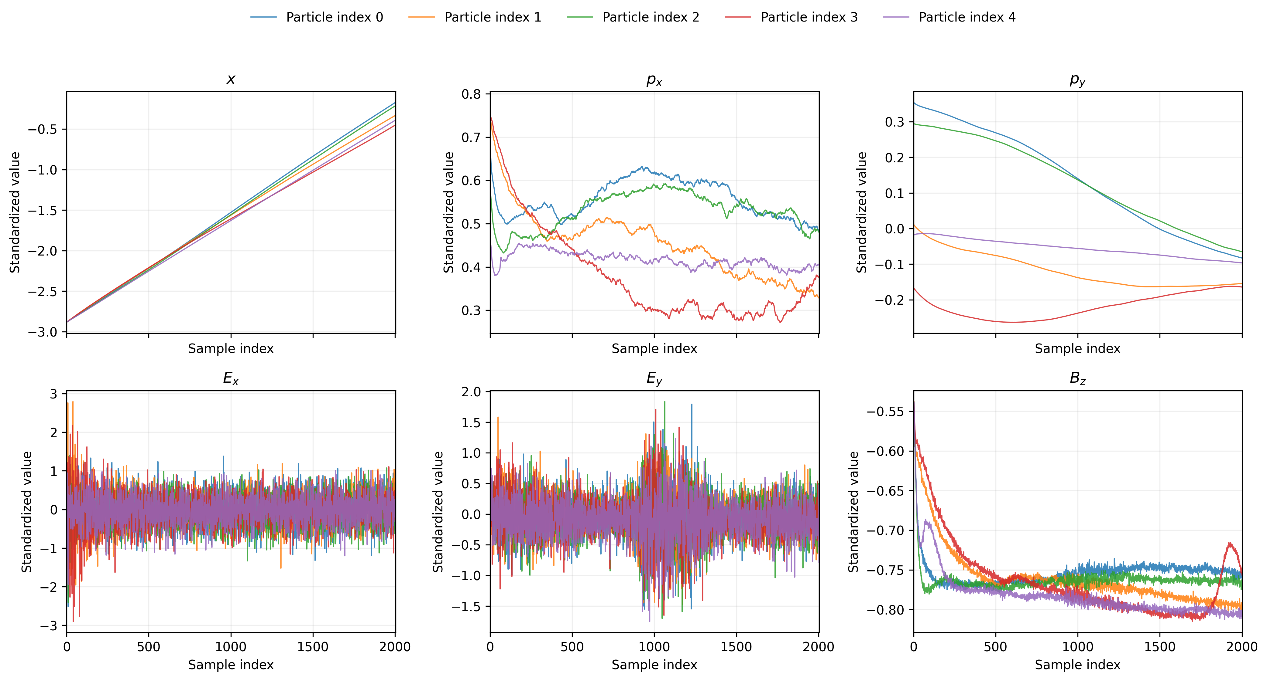
\includegraphics[width=\linewidth,height=0.58\textheight,keepaspectratio]{figures/time-series.png}
      \par\scriptsize Standardized examples; each color denotes one particle across channels.
  \end{columns}
  \vspace{0.2em}
  \centering\small Channels: \(x,\ p_x,\ p_y,\ E_x,\ E_y,\ B_z\). The available \(p_z\) channel is not used.
\end{frame}

\begin{frame}{Preprocessing: preserve correspondence, balance scale}
  \begin{enumerate}
    \item Select every third recorded sample: \(6{,}010\rightarrow2{,}004\) time points.
    \item Apply identical time indices to all particles and all six channels.
    \item Standardize each channel using statistics across the available dataset.
    \item Construct either standardized time-series inputs or six-channel spectrogram inputs.
  \end{enumerate}
  \vspace{0.5em}
  \begin{alertblock}{Evaluation scope}
    Because preprocessing statistics use the full dataset, reported scores are internal clustering assessments, not independent test-set generalization results.
  \end{alertblock}
\end{frame}

\begin{frame}{From time series to multichannel spectrograms}
  \begin{columns}[T,onlytextwidth]
    \column{.39\textwidth}
      \begin{itemize}
        \item Short-time Fourier magnitude for each standardized channel
        \item Window: 256 samples; hop: 128 samples
        \item Log compression: \(S_{\log}=\log(1+S)\)
        \item Native grid: \(129\times14\); resized to \(33\times60\)
        \item Standardize each channel; stack into \(6\times33\times60\)
      \end{itemize}
      \vspace{0.3em}\scriptsize Resizing creates a fixed input shape; it does not add independent signal information.
    \column{.59\textwidth}
      \centering
      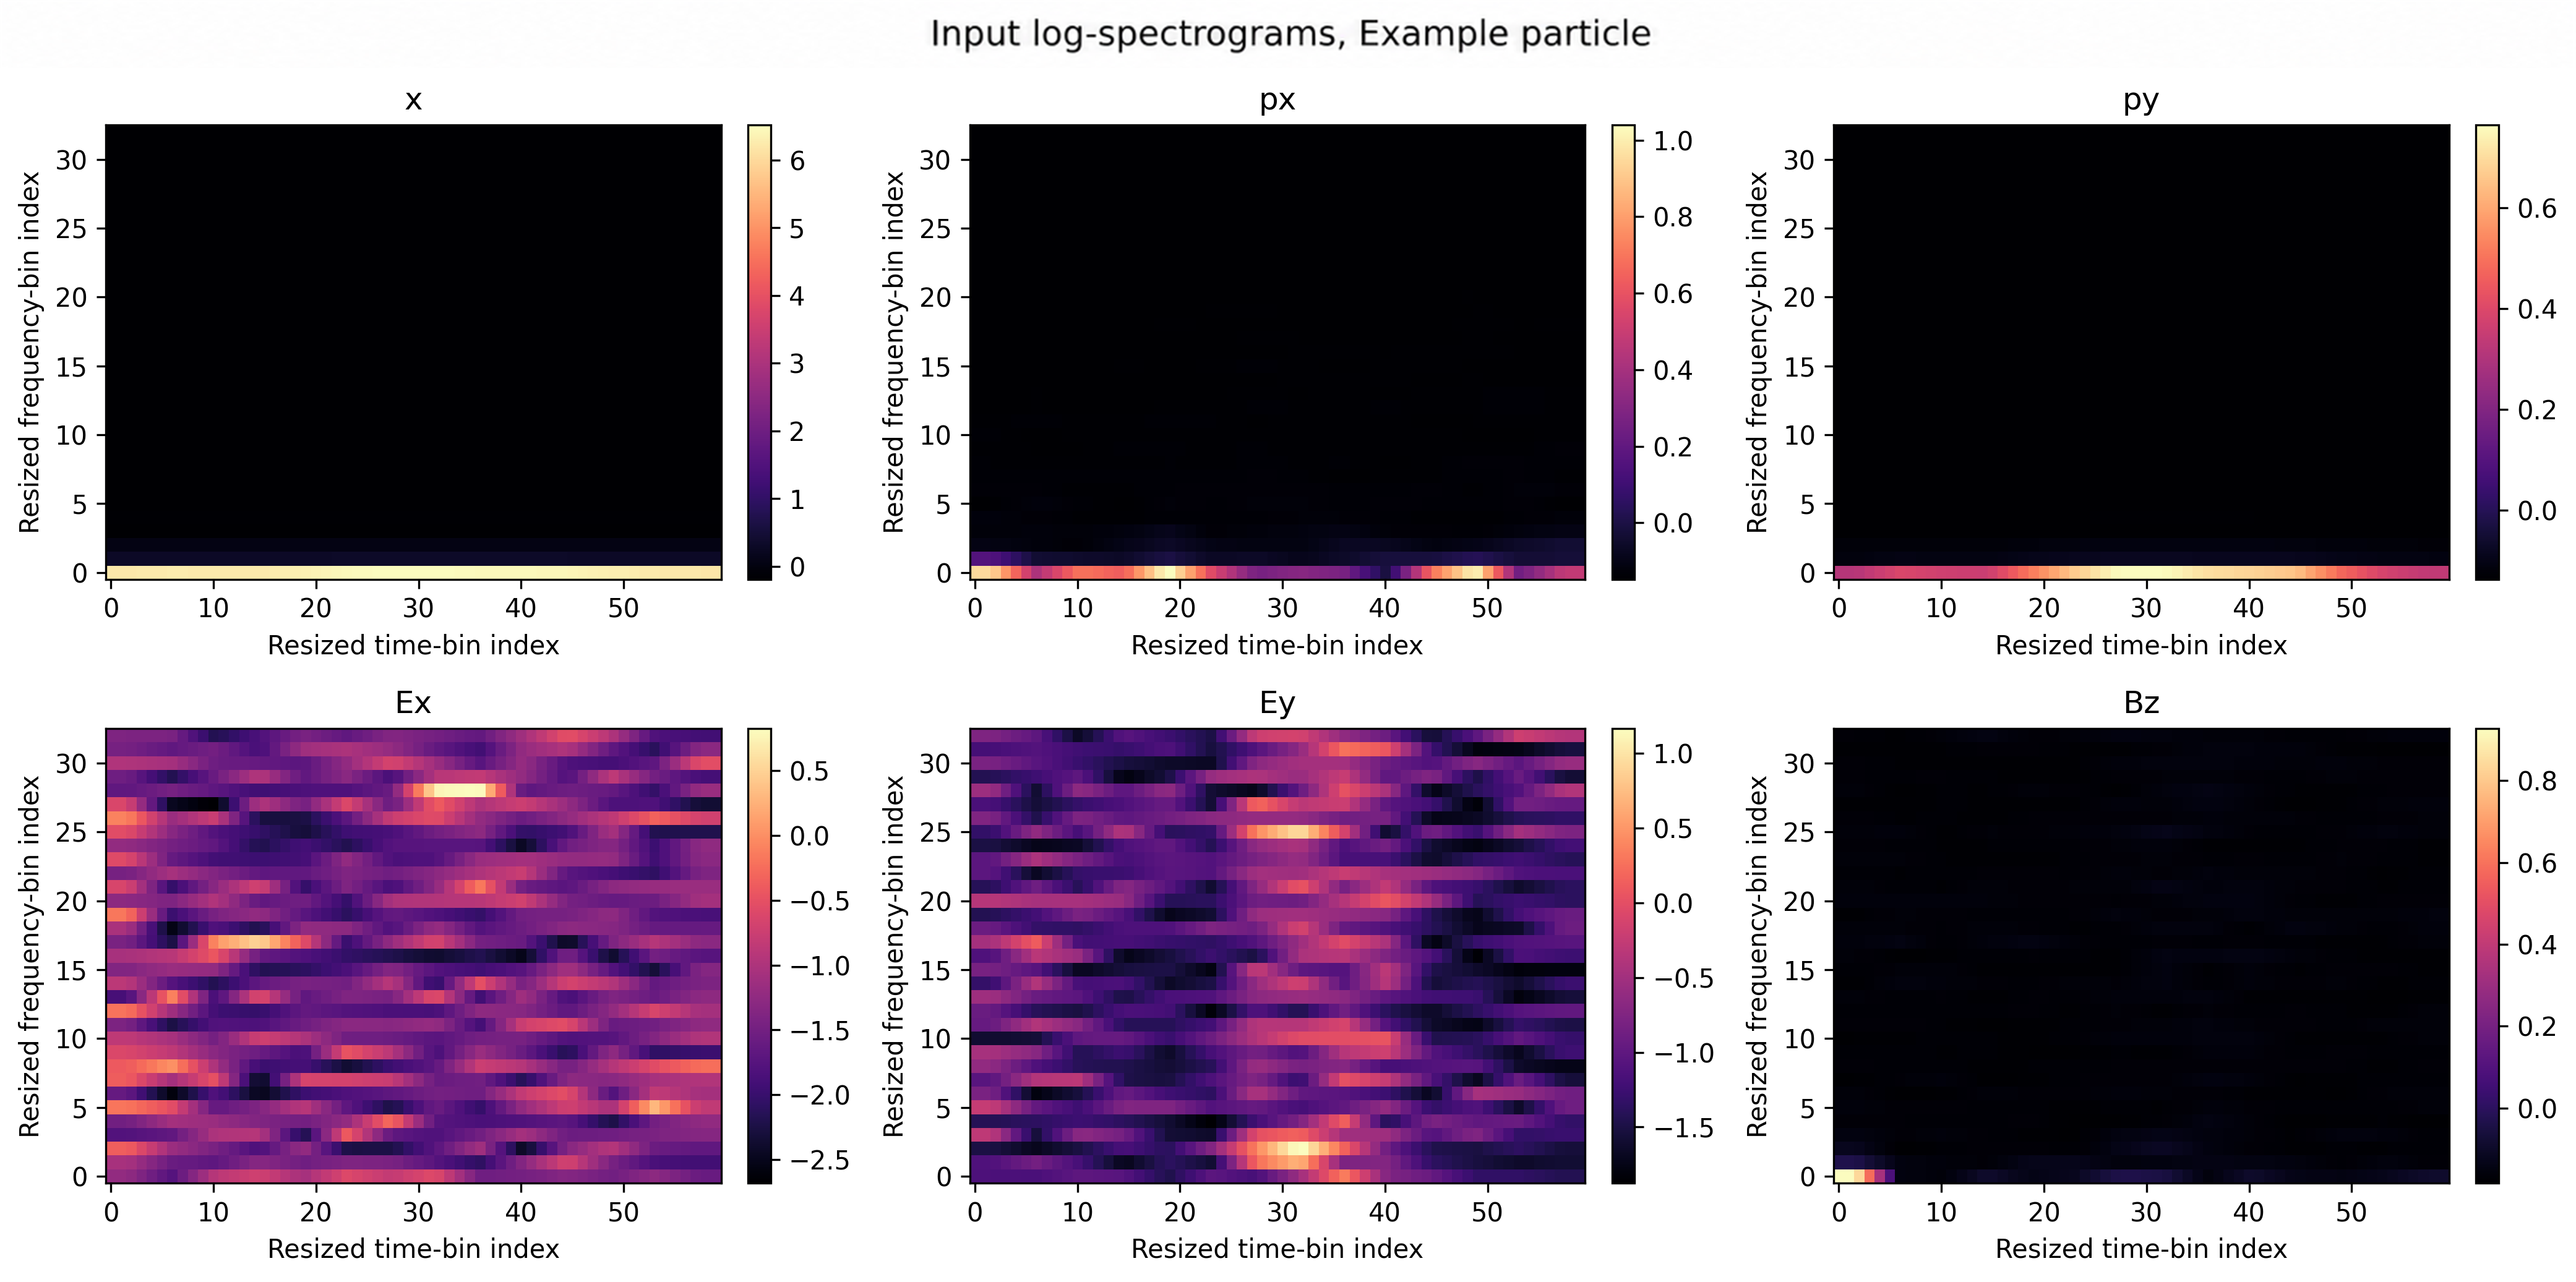
\includegraphics[width=\linewidth,height=0.68\textheight,keepaspectratio]{figures/input-log-spectrogram-example.png}
      \par\scriptsize Example six-channel log-spectrogram input.
  \end{columns}
\end{frame}

\begin{frame}{End-to-end workflow}
  \begin{center}
    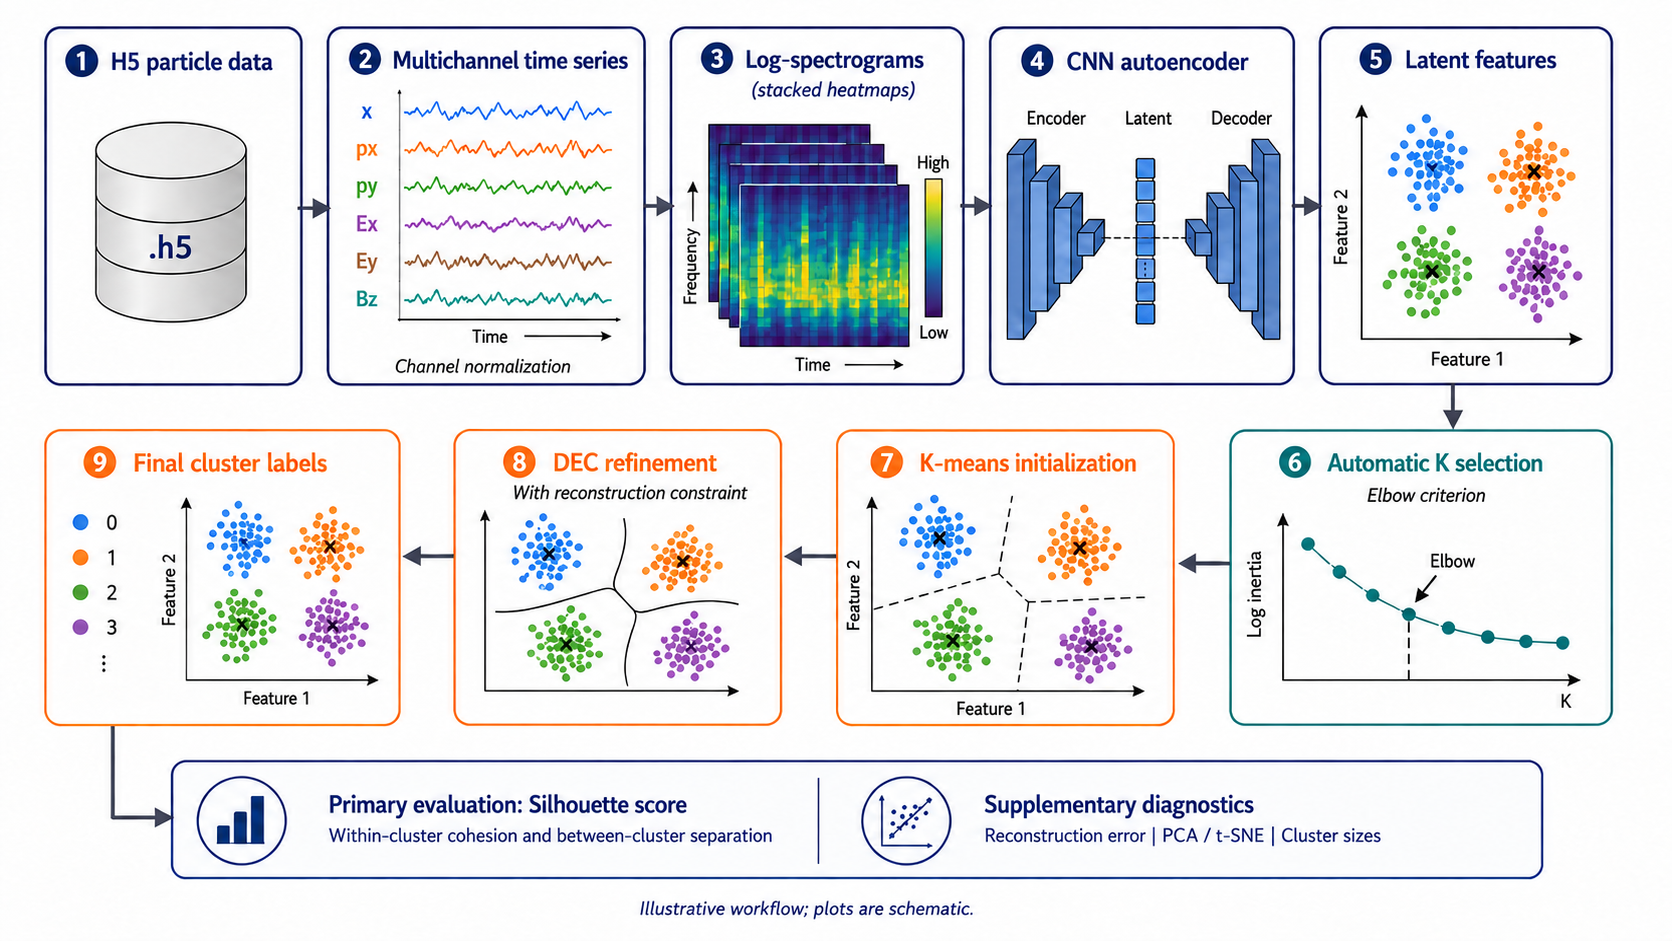
\includegraphics[width=.88\linewidth,height=.72\textheight,keepaspectratio]{figures/workflow-no-trajectories.png}
  \end{center}
  \vspace{-0.3em}
  \centering\small The spectrogram CNN + DEC pipeline is the principal method; PCA + K-means and 1D CNN + DEC serve as references.
\end{frame}

\begin{frame}{Representation learning with a convolutional autoencoder}
  \begin{columns}[T,onlytextwidth]
    \column{.54\textwidth}
      \begin{itemize}
        \item Four 2D convolutional encoder layers: 8, 16, 32, and 64 channels
        \item Compress each \(6\times33\times60\) input to a 32-dimensional code \(z_i\)
        \item Decoder reconstructs the input spectrogram
        \item Pretraining minimizes channel-weighted reconstruction error
      \end{itemize}
      \begin{block}{Why pretrain?}
        Learn a compact representation before introducing cluster assignments.
      \end{block}
    \column{.44\textwidth}
      \centering
      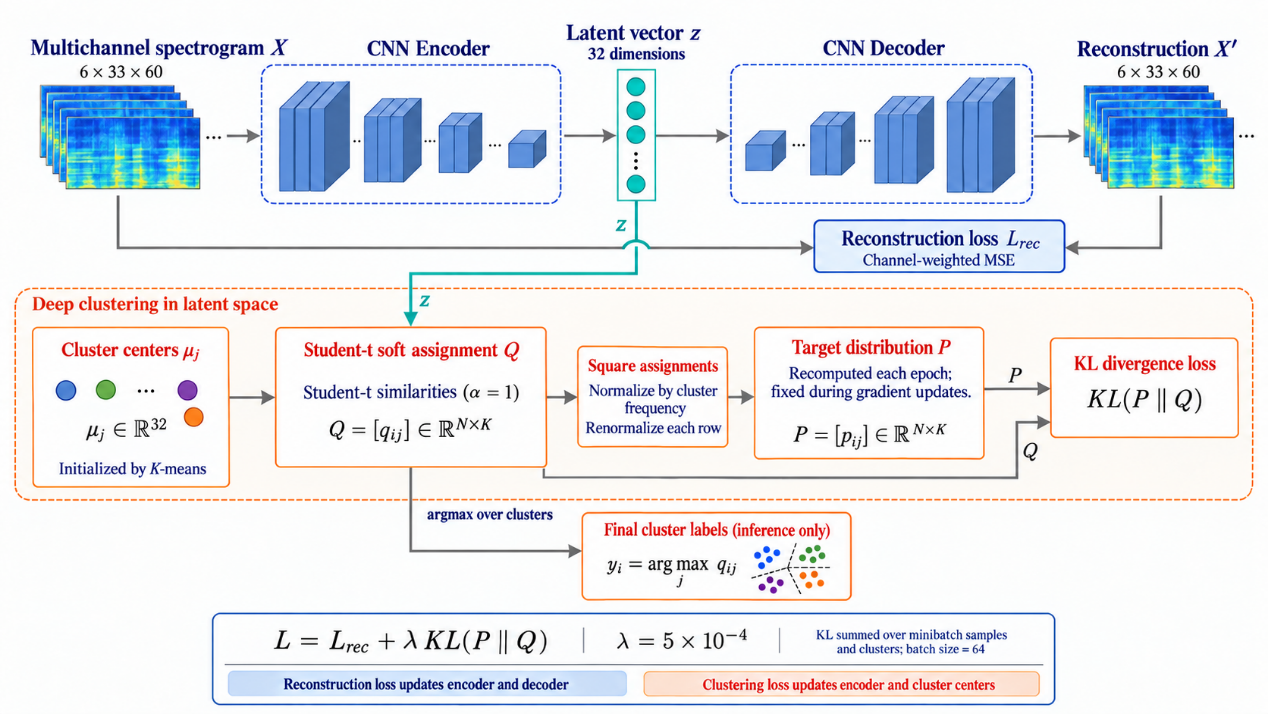
\includegraphics[width=\linewidth,height=.58\textheight,keepaspectratio]{figures/architecture.png}
      \par\scriptsize Encoder, decoder, and reconstruction-constrained clustering.
  \end{columns}
\end{frame}

\begin{frame}{DEC refinement: jointly shape features and clusters}
  Given latent point \(z_i\) and cluster center \(\mu_j\), DEC computes a soft assignment \(q_{ij}\), then sharpens assignments into a target distribution \(p_{ij}\).
  \begin{equation*}
    q_{ij}\propto\left(1+\frac{\lVert z_i-\mu_j\rVert^2}{\alpha}\right)^{-(\alpha+1)/2},\qquad
    p_{ij}\propto\frac{q_{ij}^2}{\sum_i q_{ij}},\quad \alpha=1.
  \end{equation*}
  \begin{block}{Joint objective}
    \[
      L=L_{\mathrm{recon}}+\lambda L_{\mathrm{cluster}},
      \qquad L_{\mathrm{cluster}}=\mathrm{KL}(P\Vert Q),
      \qquad \lambda=5\times10^{-4}.
    \]
  \end{block}
  \small K-means initializes five centers. The reconstruction term helps retain information about the input while the latent assignments are refined.
\end{frame}

\begin{frame}{Selecting the number of clusters}
  \begin{columns}[T,onlytextwidth]
    \column{.5\textwidth}
      \centering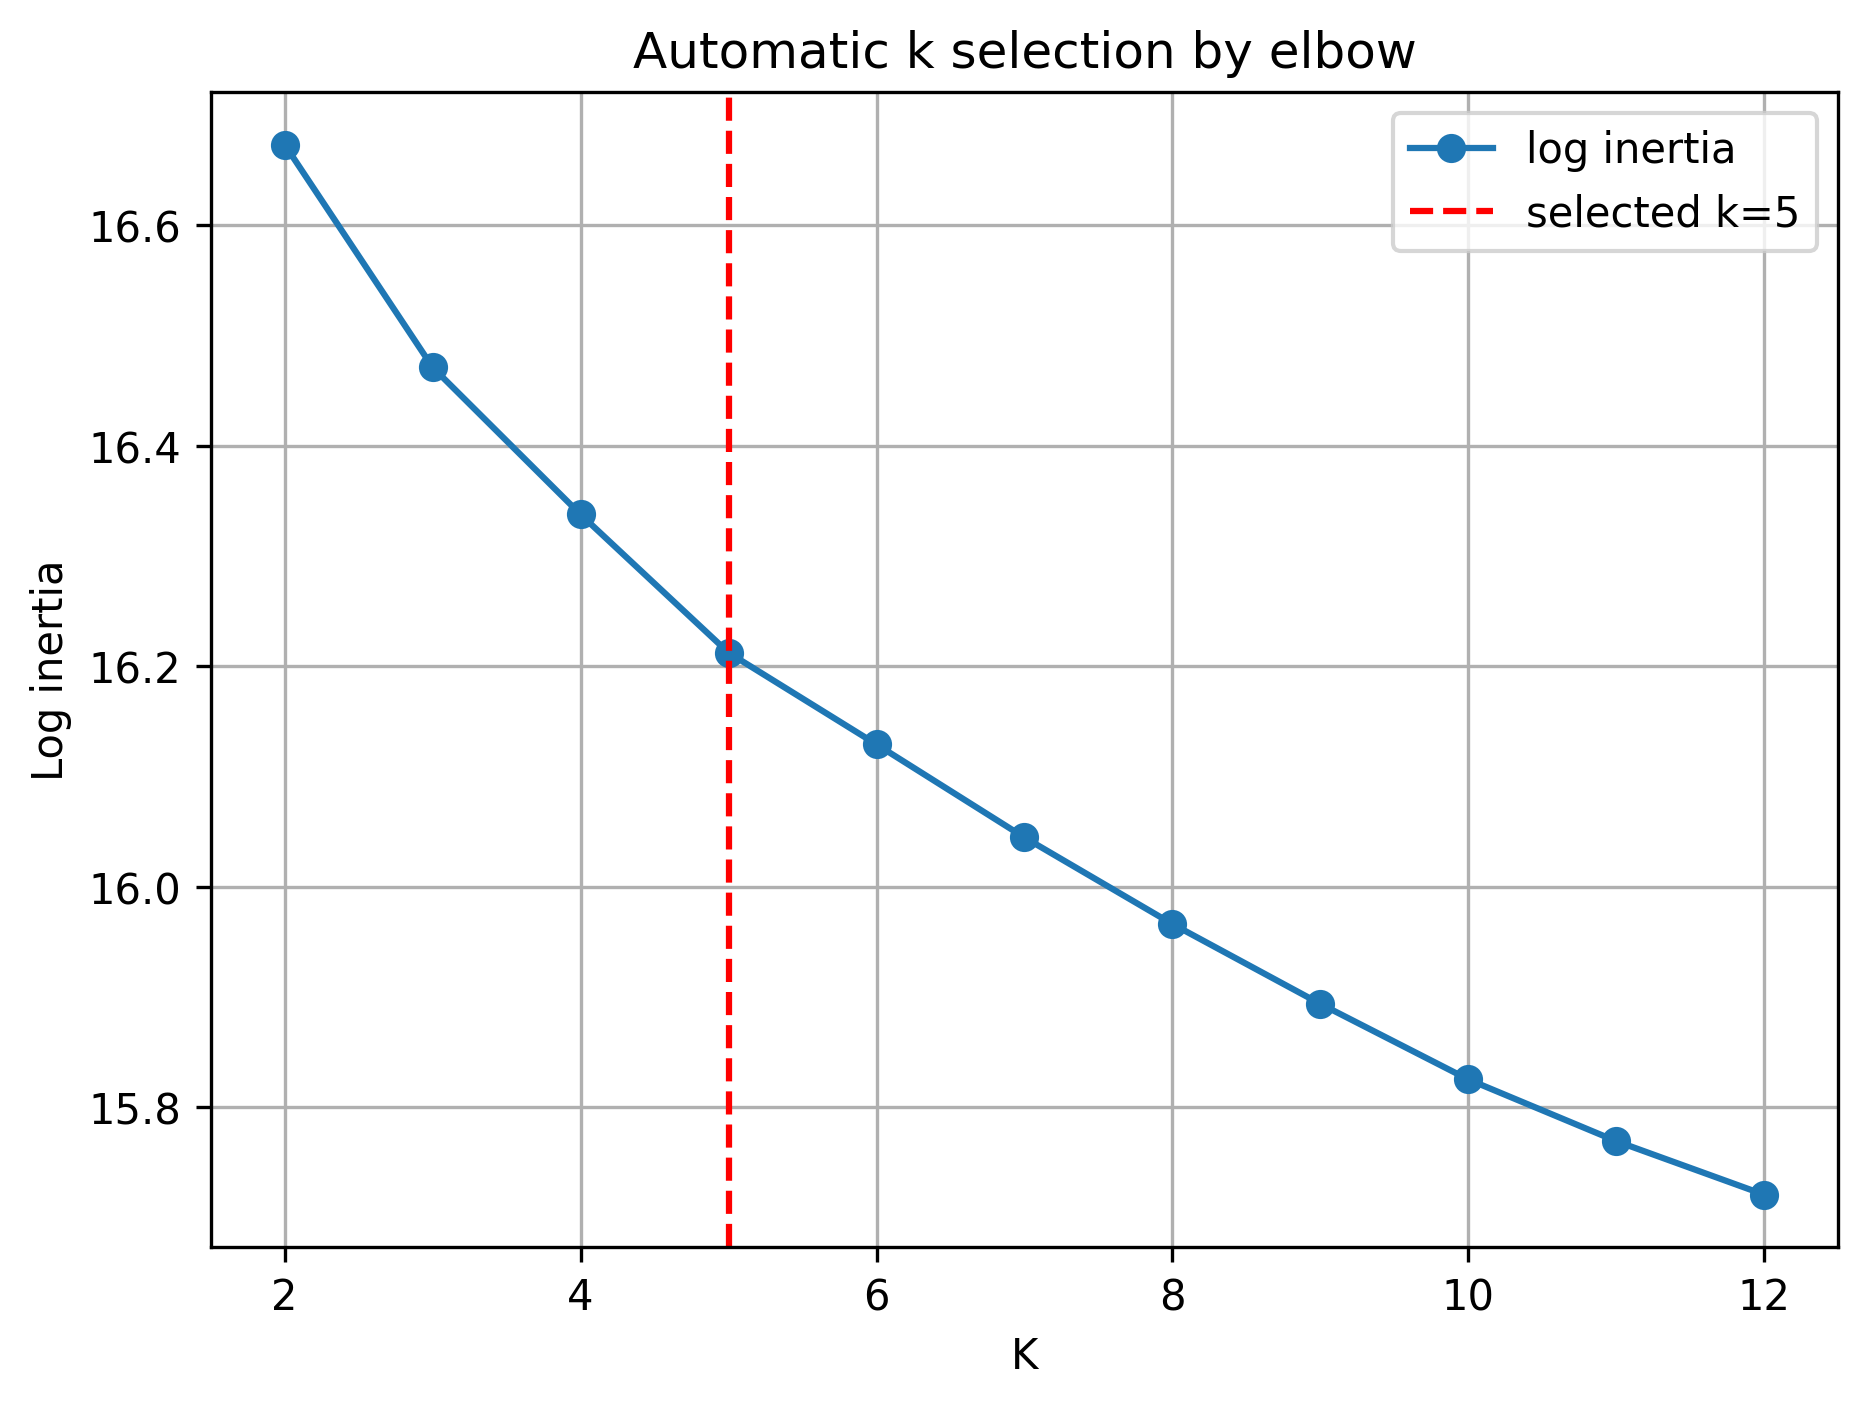
\includegraphics[width=\linewidth,height=.56\textheight,keepaspectratio]{figures/cluster-count-elbow.png}
      \par\scriptsize (a) Log-inertia elbow criterion.
    \column{.5\textwidth}
      \centering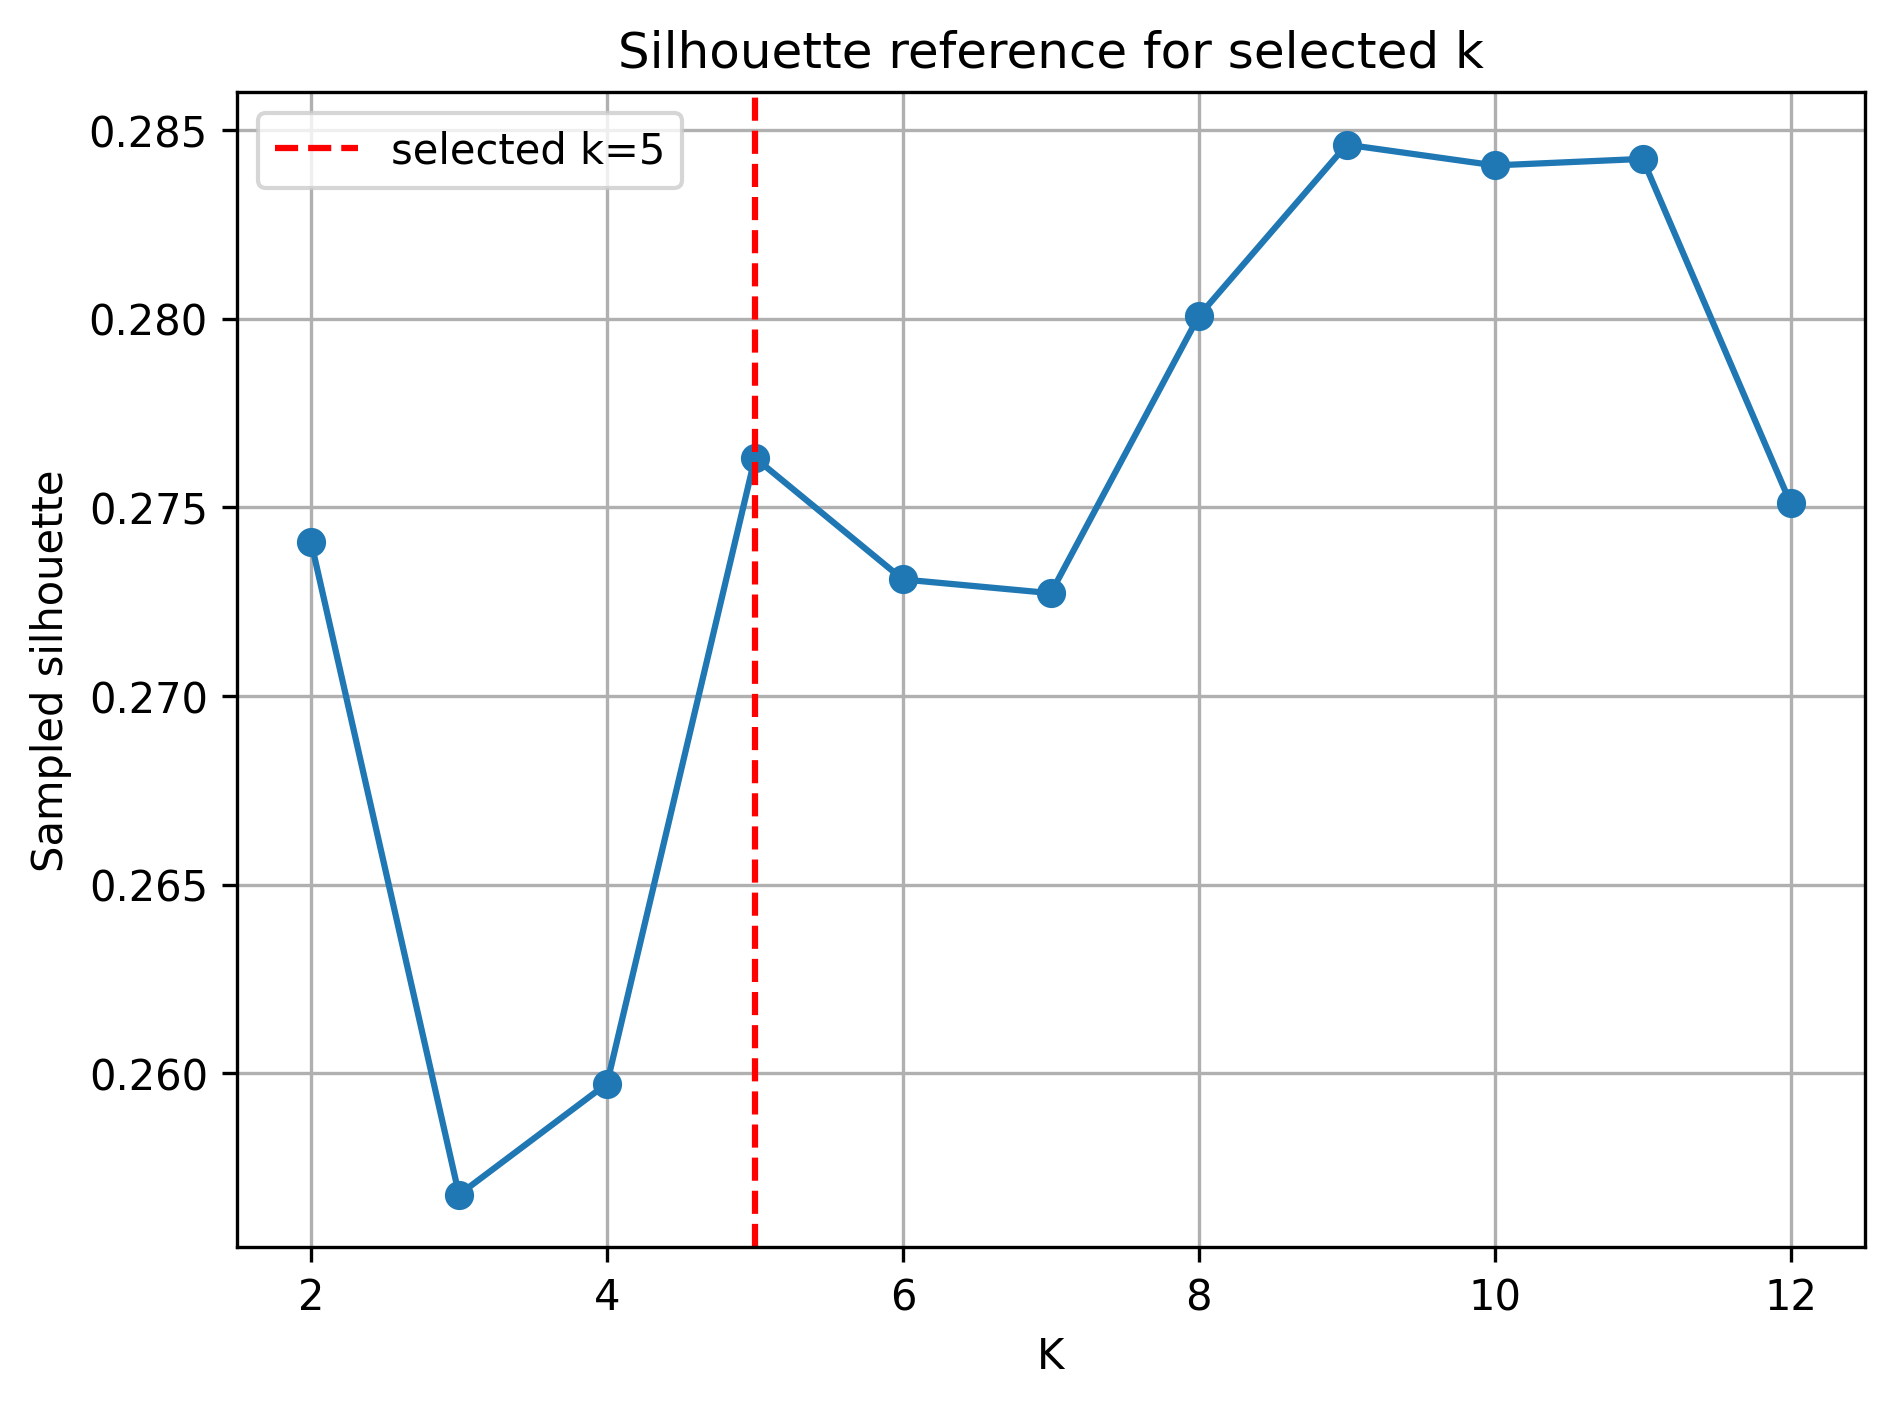
\includegraphics[width=\linewidth,height=.56\textheight,keepaspectratio]{figures/cluster-count-silhouette.png}
      \par\scriptsize (b) Silhouette values shown for reference.
  \end{columns}
  \vspace{0.4em}
  \begin{alertblock}{Decision}
    The normalized elbow criterion selects \(K=5\) from candidates \(K=2,\ldots,12\). The silhouette maximum is not used to choose \(K\).
  \end{alertblock}
\end{frame}

\begin{frame}{Experimental comparison}
  \begin{table}
    \centering\small
    \begin{tabularx}{.96\linewidth}{@{}lXX@{}}
      \toprule
      Method & Input & Representation and clustering \\
      \midrule
      PCA + K-means & Six-channel spectrogram & Flatten, PCA to 32D, K-means \\
      1D CNN + DEC & Standardized time series & 1D autoencoder, 32D, DEC \\
      Spectrogram CNN + DEC & Six-channel spectrogram & 2D autoencoder, 32D, DEC \\
      \bottomrule
    \end{tabularx}
  \end{table}
  \begin{itemize}
    \item Same 12,800-particle dataset; five clusters for all methods.
    \item Silhouette computed on the same 10,000 particles with Euclidean distance.
    \item Each method is scored in its own 32-dimensional representation space.
  \end{itemize}
\end{frame}

\begin{frame}{Main result: strongest internal silhouette for spectrogram CNN + DEC}
  \begin{columns}[T,onlytextwidth]
    \column{.61\textwidth}
      \begin{table}
        \centering\large
        \begin{tabular}{@{}lr@{}}
          \toprule
          Method & Silhouette \\
          \midrule
          PCA + K-means & 0.29957 \\
          1D CNN + DEC & 0.79637 \\
          \textbf{Spectrogram CNN + DEC} & \textbf{0.87985} \\
          \bottomrule
        \end{tabular}
      \end{table}
      \begin{block}{Observed difference}
        Spectrogram CNN + DEC exceeds the 1D CNN + DEC score by 0.08348 in this experiment.
      \end{block}
    \column{.36\textwidth}
      \vspace{0.7em}
      \centering\Large\color{SorbonneNavy}\textbf{0.87985}\par
      \small best score among tested configurations\par\vspace{1em}
      \footnotesize\color{black}Internal metric in each method's own latent space; not classification accuracy or a direct comparison in original trajectory space.
  \end{columns}
\end{frame}

\begin{frame}{Training diagnostics: optimization and monitoring}
  \begin{columns}[T,onlytextwidth]
    \column{.49\textwidth}
      \centering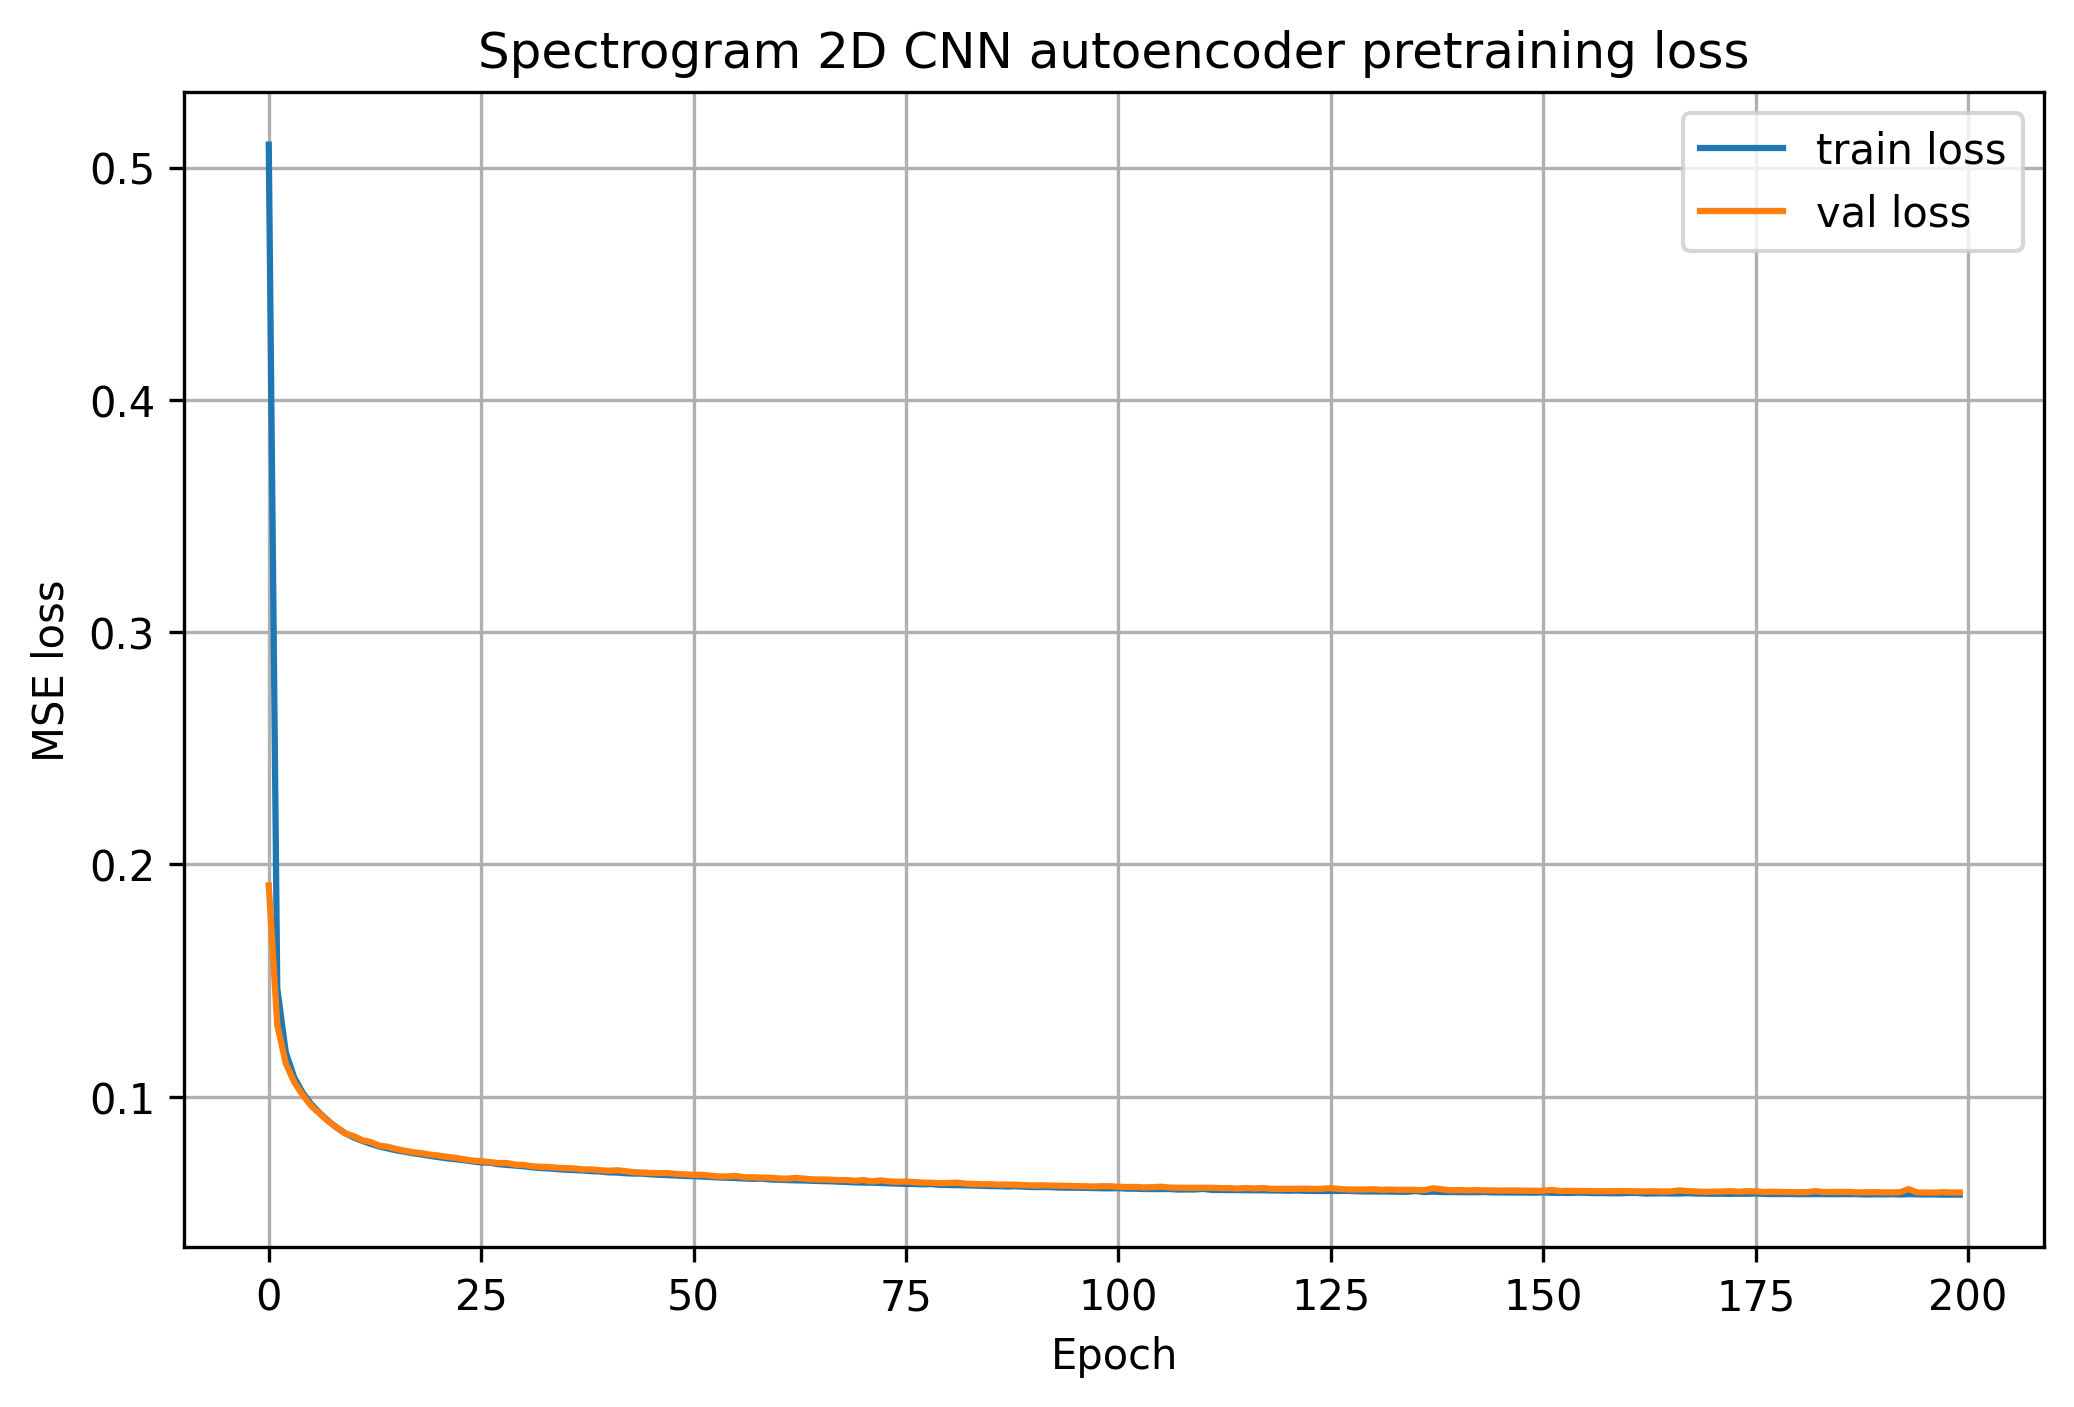
\includegraphics[width=\linewidth,height=.48\textheight,keepaspectratio]{figures/ae-pretraining-loss.png}
      \par\scriptsize Autoencoder pretraining: training and validation reconstruction loss.
    \column{.49\textwidth}
      \centering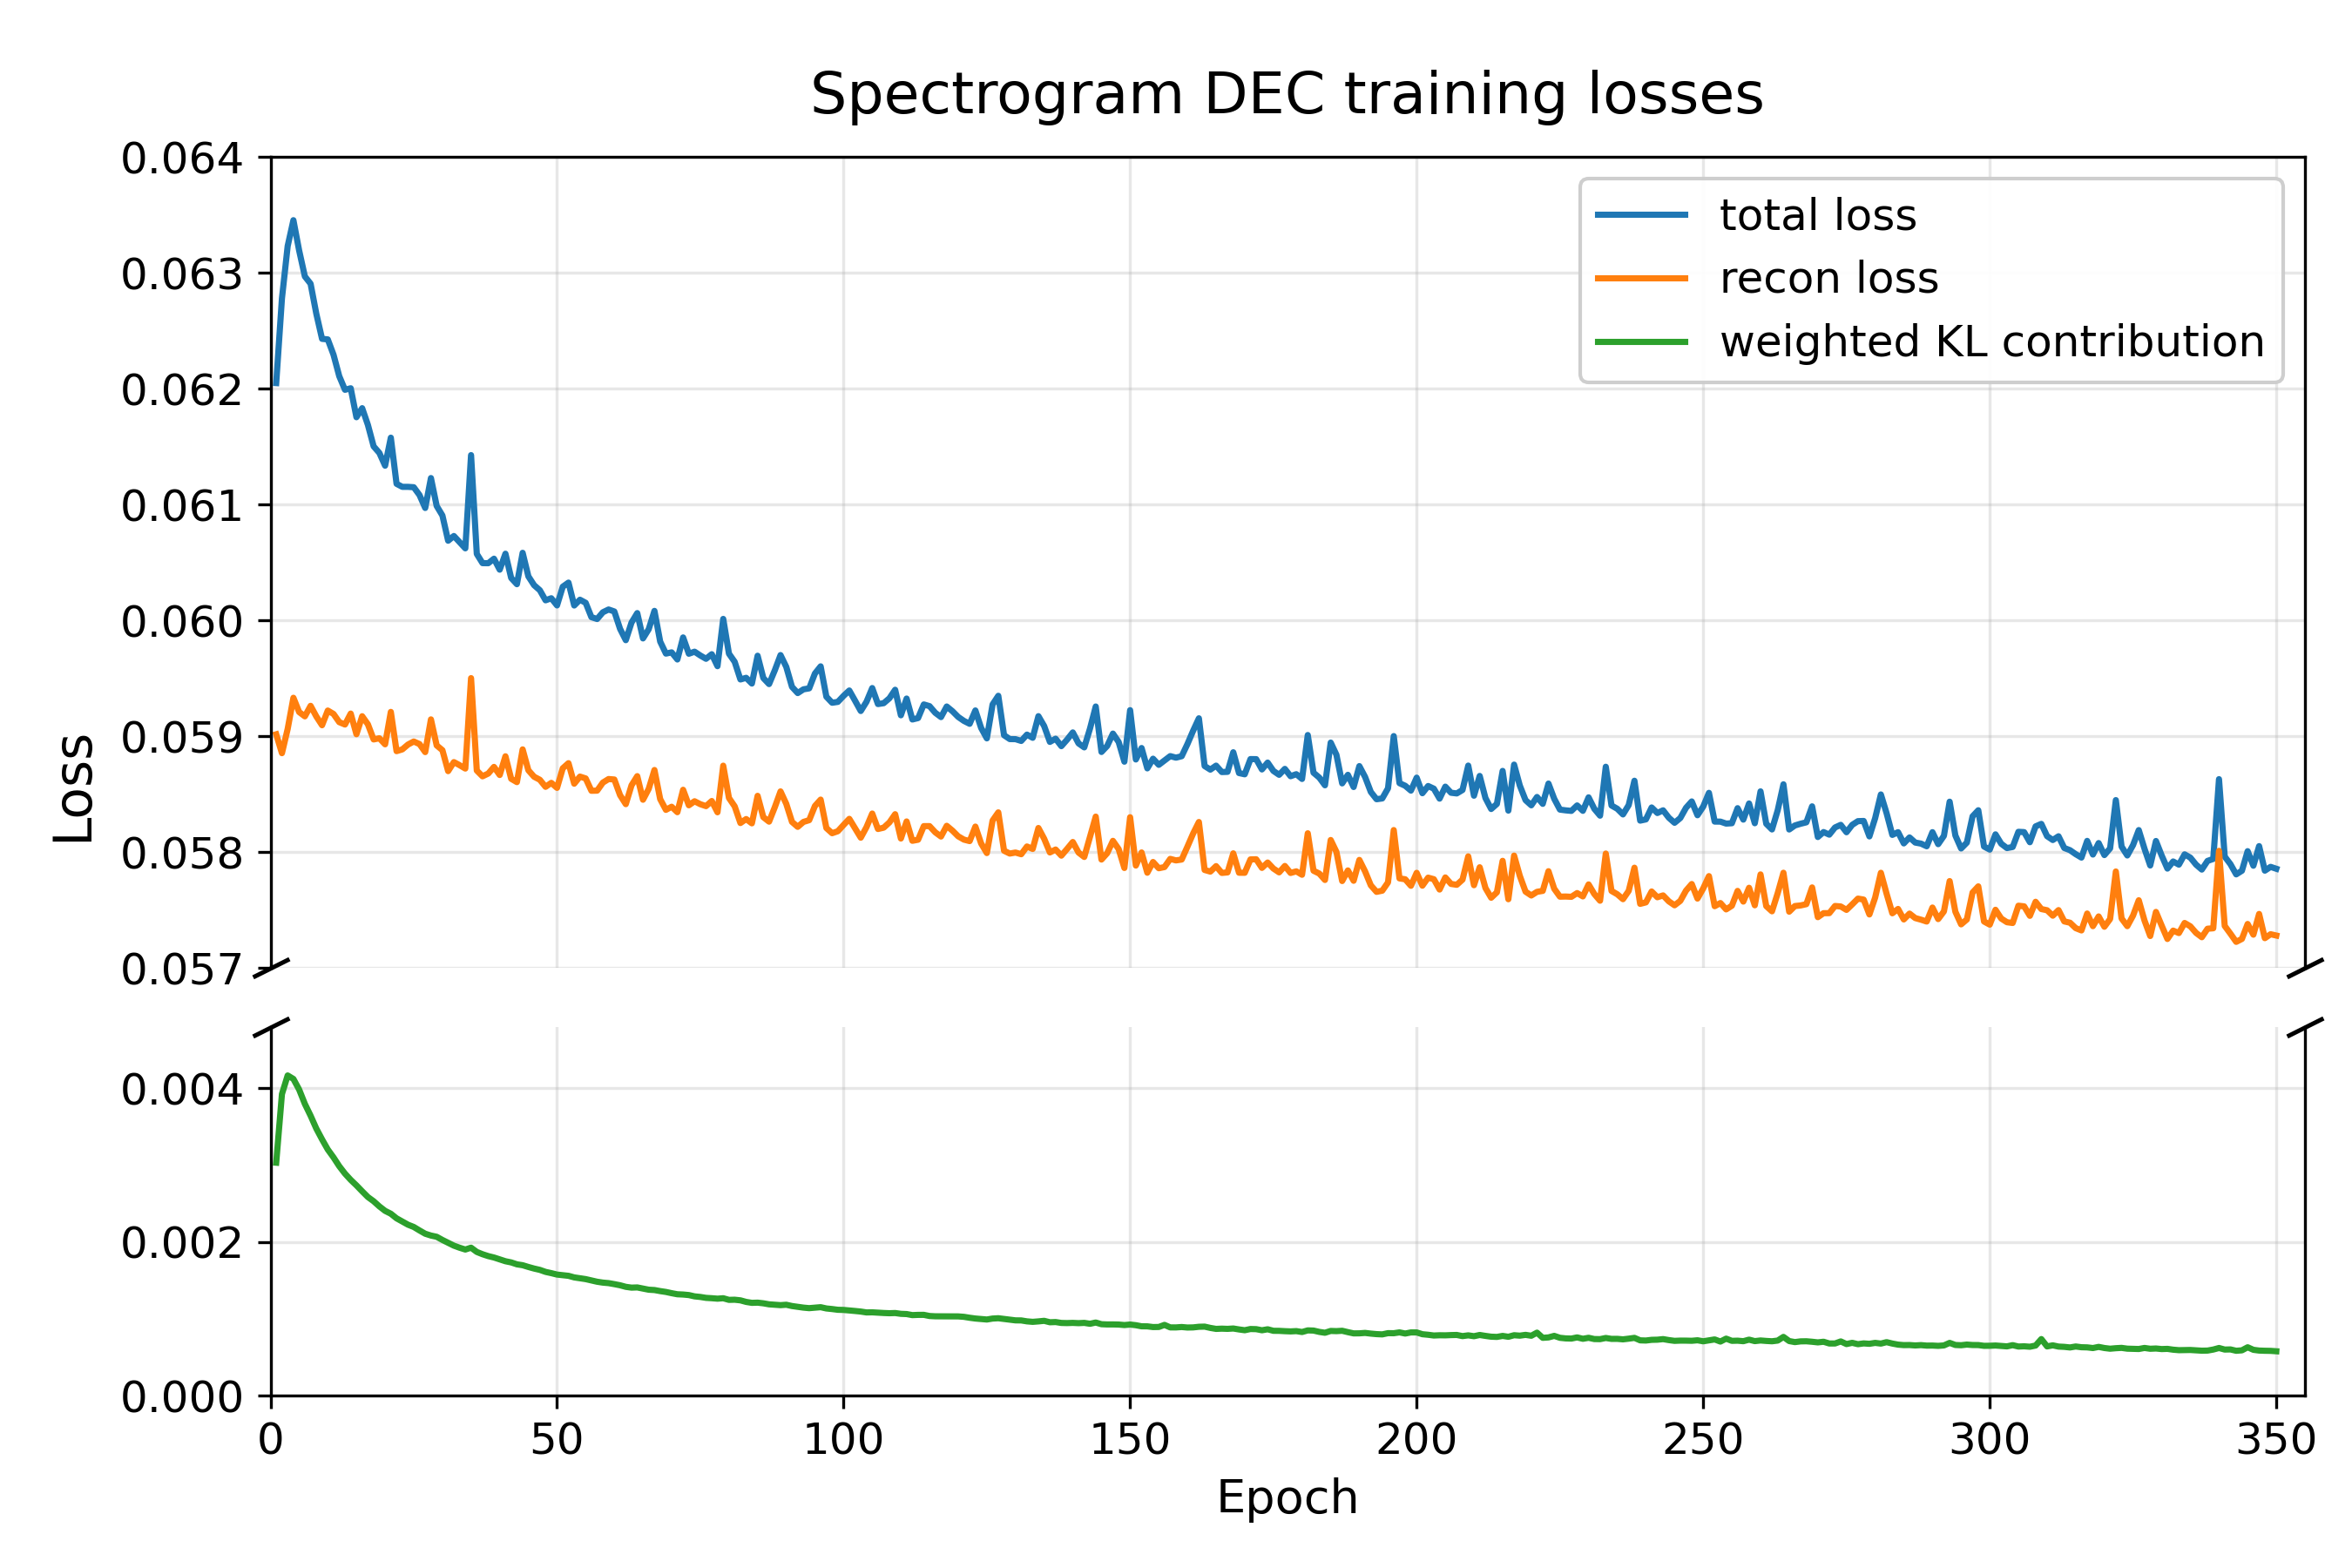
\includegraphics[width=\linewidth,height=.48\textheight,keepaspectratio]{figures/dec-training-loss-zoomed.png}
      \par\scriptsize DEC refinement: reconstruction, clustering, and total losses.
  \end{columns}
  \vspace{0.3em}
  \centering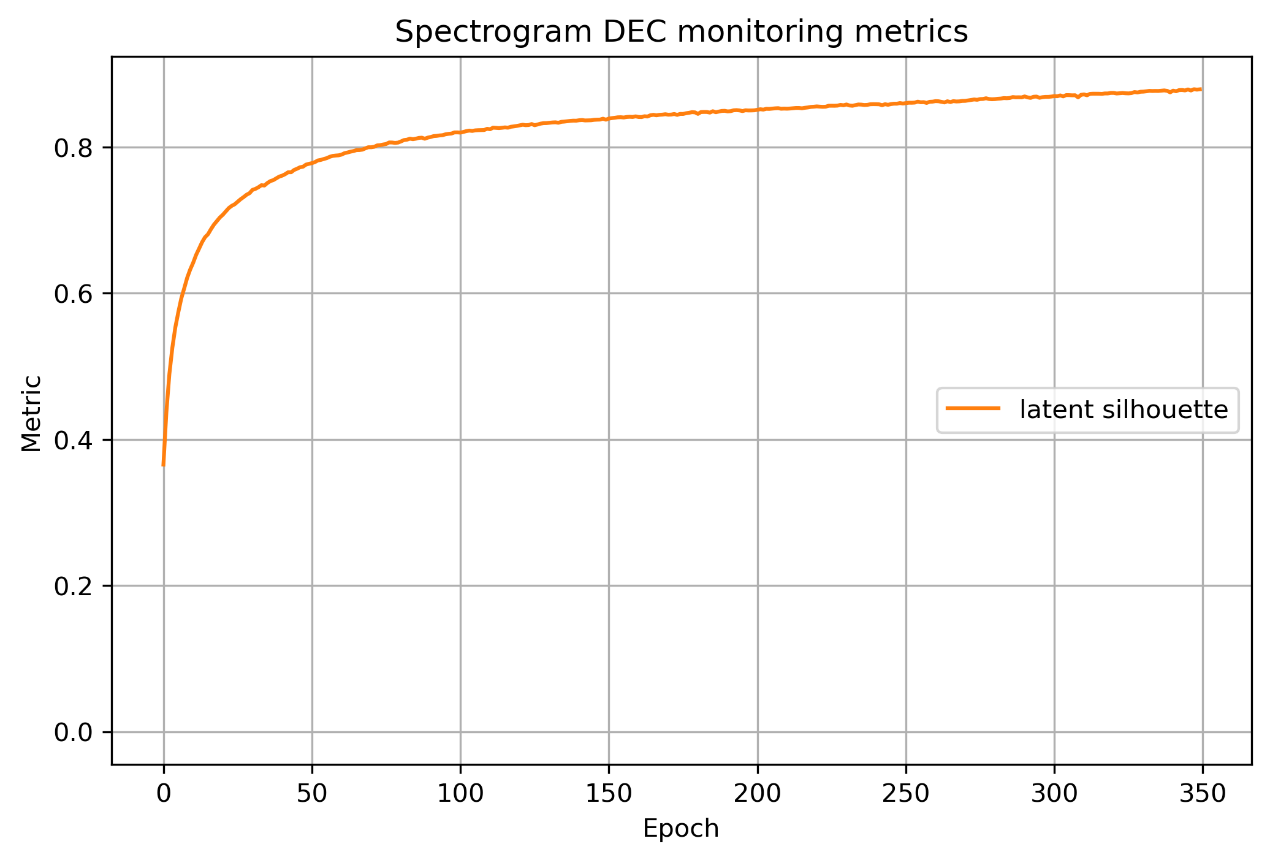
\includegraphics[width=.43\linewidth,height=.22\textheight,keepaspectratio]{figures/dec-silhouette.png}
  \hspace{0.5em}\parbox[b]{.45\linewidth}{\scriptsize Silhouette is monitored on 5,000 particles during refinement; final evaluation uses 10,000. Training was run for 350 DEC epochs.}
\end{frame}

\begin{frame}{Reconstruction: a representation diagnostic}
  \begin{columns}[T,onlytextwidth]
    \column{.55\textwidth}
      \centering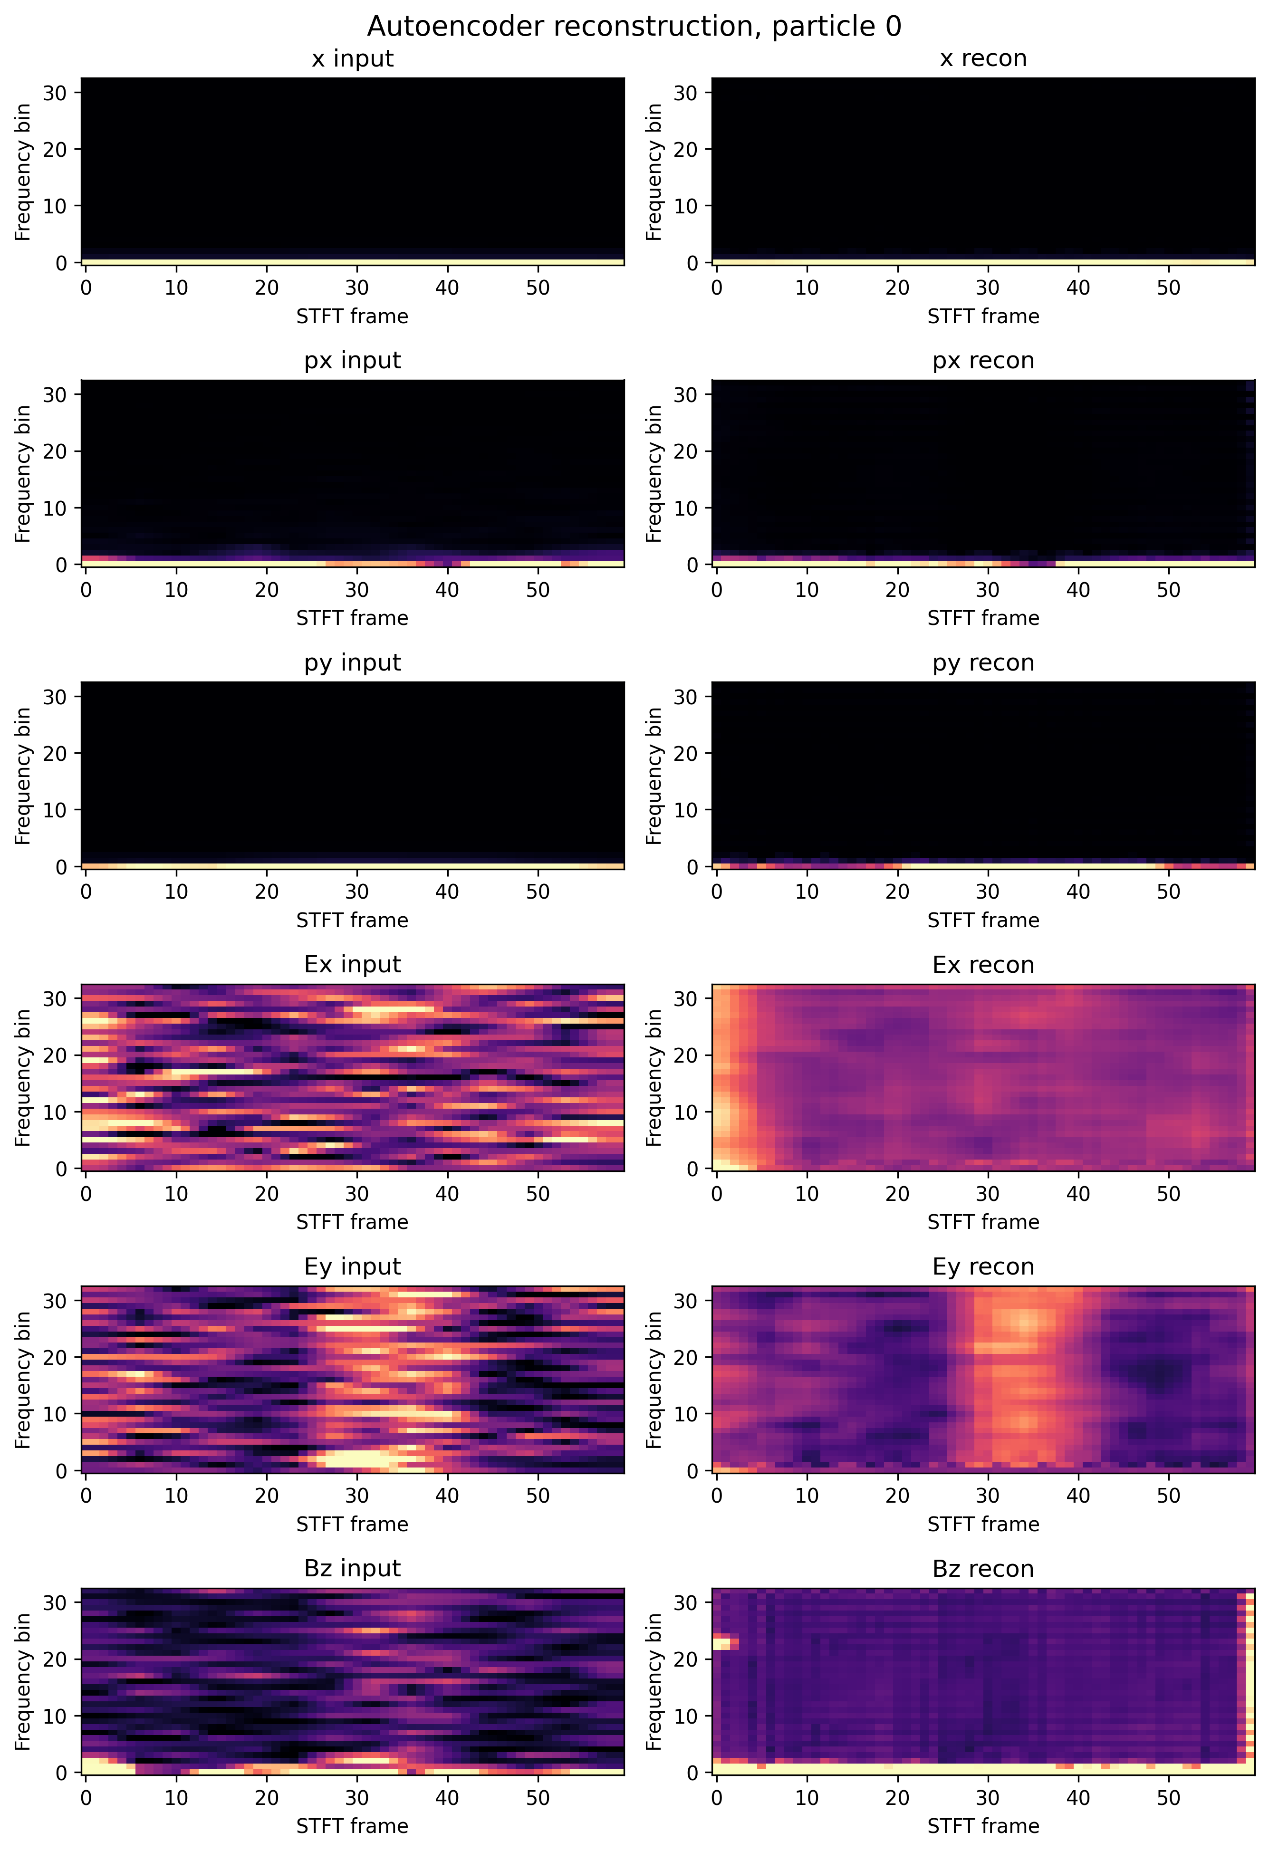
\includegraphics[width=\linewidth,height=.75\textheight,keepaspectratio]{figures/reconstruction.png}
    \column{.41\textwidth}
      \begin{block}{What this checks}
        Can the pretrained autoencoder reproduce the broad channel-wise time--frequency patterns?
      \end{block}
      \begin{itemize}
        \item Rows correspond to \(x,p_x,p_y,E_x,E_y,B_z\).
        \item Reconstruction loss measures input fidelity.
        \item It is a supplementary diagnostic, not a clustering-quality score.
      \end{itemize}
  \end{columns}
\end{frame}

\begin{frame}{Final latent-space visualization}
  \begin{columns}[T,onlytextwidth]
    \column{.5\textwidth}
      \centering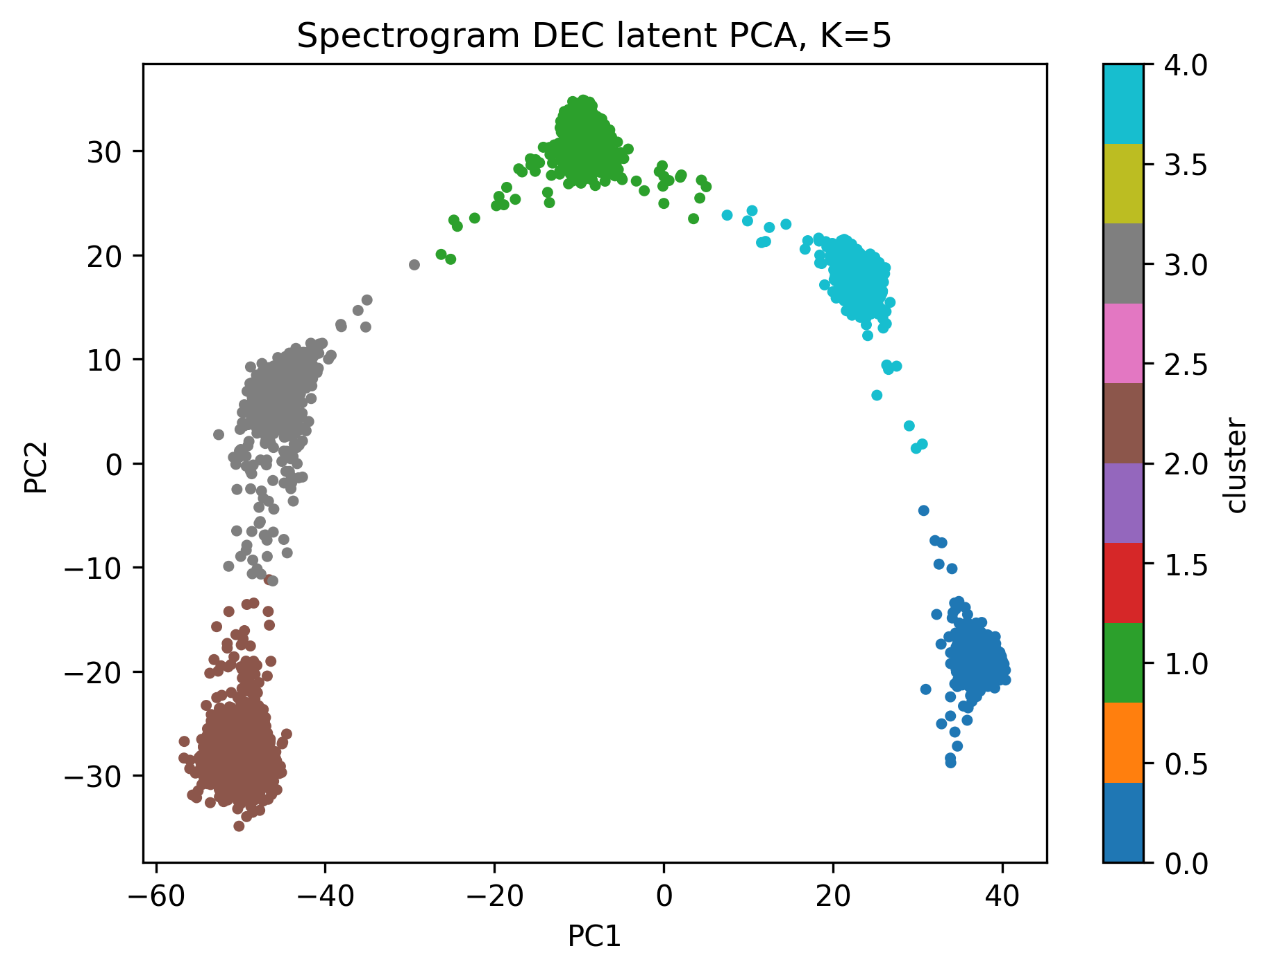
\includegraphics[width=\linewidth,height=.58\textheight,keepaspectratio]{figures/latent-pca.png}
      \par\scriptsize PCA projection.
    \column{.5\textwidth}
      \centering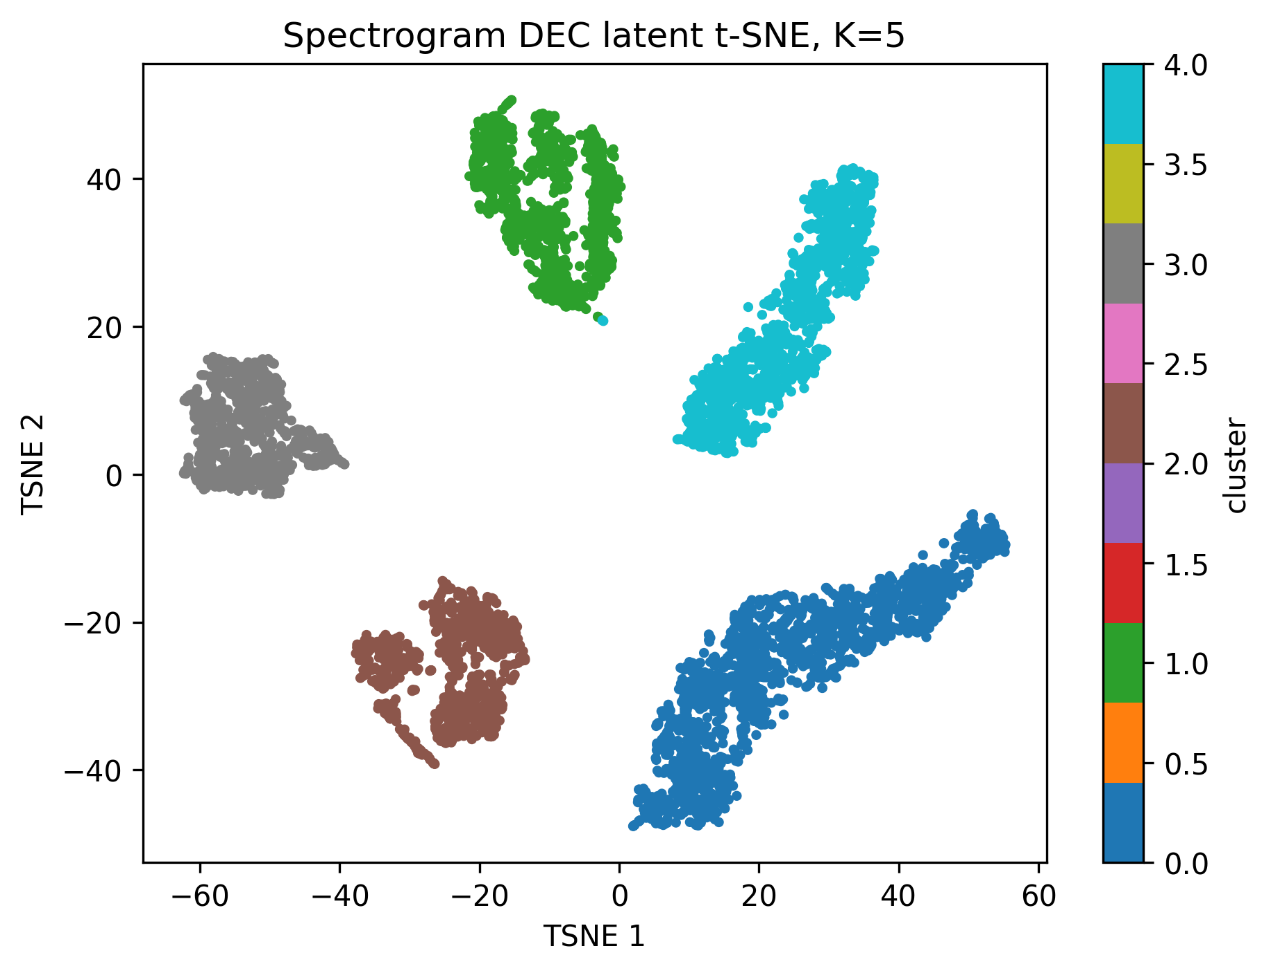
\includegraphics[width=\linewidth,height=.58\textheight,keepaspectratio]{figures/latent-tsne.png}
      \par\scriptsize t-SNE projection.
  \end{columns}
  \vspace{0.35em}
  \centering\small Colors show the five final labels. Clustering and silhouette are computed in 32D, not in these 2D projections.
\end{frame}

\begin{frame}{Five groups: distribution across all particles}
  \begin{columns}[T,onlytextwidth]
    \column{.58\textwidth}
      \begin{table}
        \centering\large
        \begin{tabular}{@{}lrr@{}}
          \toprule
          Cluster & Particles & Share \\
          \midrule
          C0 & 3,884 & 30.34\% \\
          C1 & 2,314 & 18.08\% \\
          C2 & 2,068 & 16.16\% \\
          C3 & 1,818 & 14.20\% \\
          C4 & 2,716 & 21.22\% \\
          \midrule
          Total & 12,800 & 100.00\% \\
          \bottomrule
        \end{tabular}
      \end{table}
    \column{.37\textwidth}
      \begin{block}{Interpretation}
        All clusters are nonempty and contain substantial numbers of particles.
      \end{block}
      \small Cluster indices are identifiers assigned by the algorithm, not physical classes. Size alone does not validate a partition.
  \end{columns}
\end{frame}

\begin{frame}{Computational cost and scale-up scenario}
  \begin{columns}[T,onlytextwidth]
    \column{.48\textwidth}
      \begin{block}{Measured: 12,800 particles}
        \begin{itemize}
          \item Spectrogram CNN + DEC: \textbf{524.62 s}
          \item 1D CNN + DEC: \textbf{405.19 s}
          \item NVIDIA RTX PRO 6000 Blackwell Server Edition
        \end{itemize}
      \end{block}
      \scriptsize Includes preprocessing, pretraining, 350 refinement epochs, evaluation, and figure generation.
    \column{.48\textwidth}
      \begin{block}{Linear-scaling estimate}
        \begin{itemize}
          \item 1 million particles: about \textbf{11.4 hours}
          \item 10 million particles: about \textbf{4.7 days}
        \end{itemize}
      \end{block}
      \scriptsize Projection assumes unchanged settings and per-particle dimensions. It is a rough estimate, not a benchmark at scale.
  \end{columns}
  \vspace{0.45em}
  \alert{Large-scale use would require careful data loading and memory management.}
\end{frame}

\begin{frame}{Limitations and interpretation}
  \begin{itemize}
    \item \textbf{Internal metric:} silhouette measures cohesion and separation in a chosen representation; it does not show physical ground-truth classes.
    \item \textbf{Different spaces:} each method is evaluated in its own latent space, so scores are not a common-space comparison.
    \item \textbf{Single dataset:} no independent simulation, time interval, or particle-sample validation was performed.
    \item \textbf{Representation choices:} magnitude spectrograms, resizing, selected channels, and sampling affect the discovered groups.
    \item \textbf{Scale-up:} million-particle runtimes are extrapolations under a linear assumption.
  \end{itemize}
  \vspace{0.5em}
  \begin{block}{Careful claim}
    The results support a useful way to organize these records, not a claim that the five groups are validated physical categories.
  \end{block}
\end{frame}

\begin{frame}{Conclusions and next steps}
  \begin{enumerate}
    \item A six-channel spectrogram pipeline was implemented for 12,800 PIC particle trajectories.
    \item The spectrogram CNN + DEC model learned 32D features and produced five clusters.
    \item It achieved the highest observed silhouette (0.87985) among the three tested methods, under internal evaluation.
    \item The workflow offers an indexing and exploration tool for subsequent domain-specific analysis.
  \end{enumerate}
  \vspace{0.45em}
  \begin{alertblock}{Next steps}
    Validate across additional simulations; relate clusters to physical diagnostics; evaluate sensitivity to channels and preprocessing; improve throughput for large datasets.
  \end{alertblock}
\end{frame}

\begin{frame}[plain]
  \vfill
  \centering
  {\Huge\color{SorbonneNavy}Thank you}\par
  \vspace{1em}
  {\Large Questions and discussion}\par
  \vfill
  {\small Linshuo CHEN \quad $\vert$ \quad Supervisor: Andrea CIARDI}
\end{frame}

\end{document}